\lab{Transit Time Crossing a River}{Transit Time Crossing a River}
\label{lab:rivercrossing}
\objective{This lab discusses a classical calculus of variations problem: how is a river to be crossed in the shortest possible time? 
We will look at a numerical solution using the pseudospectral method. }
\labdependencies{SpectralMethod1}

Suppose a boat is to be rowed across a river, from a point $A$ on one side of a river ($x=-1$), to a point $B$ on the other side ($x=1$). 
Assuming the boat moves at a constant speed 1 relative to the current, how must the boat be steered to minimize the time required to cross the river? 

\begin{figure}
\centering
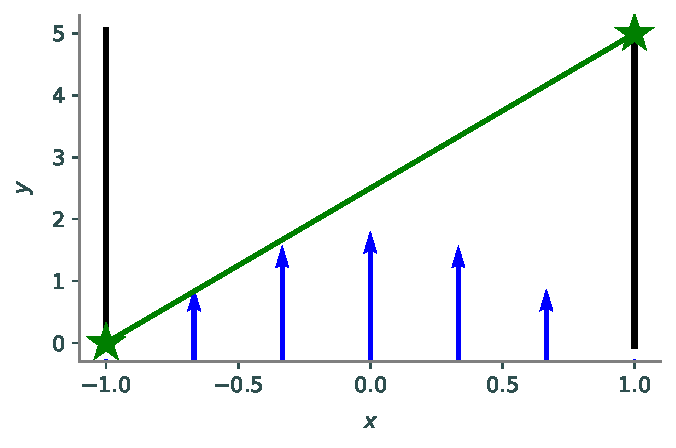
\includegraphics[width=\textwidth]{figures/rivercurrent.pdf}
\caption{The river's current, along with a possible trajectory for the boat.}
\label{fig:rivercrossing_current}
\end{figure}


Let us consider a typical trajectory for the boat as it crosses the river. 
If $T$ is the time required to cross the river, then the position $s$ of the boat at time $t$ is
\begin{align*}
	s(t) &= (x(t), y(t)), \quad t \in [0,T], \\
	s'(t) &= (x'(t), y'(t)) \\ 
	&= (\cos \theta(x(t)),\sin \theta(x(t))) + (0, c(x(t))).
\end{align*}
Here $(\cos \theta(x), \sin \theta(x))$ represents the motion of the boat due to the rower, and $(0, c(x))$ is the motion of the boat due to the current.

We can relate the angle at which the boat is steered to the graph of its trajectory by noting that 
\begin{align}
\begin{split}
	y'(x) &= \frac{y'(t)}{x'(t)} ,\\
	&= \frac{\sin \theta(x) + c(x)}{\cos \theta(x)},\\
	&= c(x)\sec \theta(x) + \tan \theta(x) .%, \\
	% &= c \sec \theta + \sqrt{\sec^2 \theta -1}.
\end{split} \label{rivercrossing:angle}
\end{align}
The time $T$ required to cross the river is given by
\begin{align}
\begin{split}
	T &= \int_{-1}^1 t'(x)\, dx, \\
	&= \int_{-1}^1 \frac{1}{x'(t)}\, dx \\ 
	&= \int_{-1}^1 \sec \theta(x)\, dx. 
\end{split}\label{rivercrossing:T}
\end{align}
We would like to find an expression for the total time $T$ required to cross the river from $A$ to $B$, in terms of the graph of the boat's trajectory. 
To derive the functional $T[y]$, we note that 
\begin{align*}
	T[y] &= \int_{-1}^1 \sec \theta(x) dx,\\
	&= \int_{-1}^1 \frac{1}{1-c(x)^2}(c(x) \tan \theta(x) + \sec \theta(x) -c(x)^2 \sec \theta(x) - c(x)\tan \theta(x))\, dx, \\
	&= \int_{-1}^1 \frac{1}{1-c(x)^2}(c(x) \tan \theta(x) + \sec \theta(x) -c(x) y'(x) )\, dx.	
\end{align*}
Since 
\begin{align*}
	c(x)\tan \theta(x) + \sec \theta(x) &= \sqrt{1 - c(x)^2 + (c(x) \sec \theta(x) + \tan \theta(x))^2},\\
	&= \sqrt{1 - c(x)^2 + (y'(x))^2},
\end{align*}
we obtain at last
\begin{align}
	T[y] &= \int_{-1}^1 \left[ \alpha(x)\sqrt{1 + (\alpha(x) y'(x))^2} - \alpha^2(x) c(x) y'(x) \right]\, dx,
\end{align}
where $\alpha(x) = (1 - c^2(x))^{-1/2}$.

\begin{problem}
Assume that the current is given by $c(x) = -\frac{7}{10}(x^2-1)$. (This function assumes, for example, that the current is faster near the center of the river.)
Write two python functions. The first should accept as arguments a function $y$, its derivative $y'$, and an $x$-value, and return $L(x,y(x),y'(x))$ (where $T[y] = \int_{-1}^1 L(x,y(x),y'(x))$). 
The second should use the first function to compute and return $T[y]$ for a given path $y(x)$.
\\ Hint: The integration for $T[y]$ can be done use an approximation method such as the midpoint method or can be done using the \li{quad} function from \li{scipy.integrate}.
\end{problem}

\begin{problem}
	Let $y(x)$ be the straight-line path between $A = (-1,0)$ and $B=(1,5)$. Numerically calculate $T[y]$ to get an upper bound on the minimum time required to cross from $A$ to $B$. Using $\eqref{rivercrossing:T}$, find a lower bound on the minimum time required to cross.
	\\Hint: If $G=\int f(x)dx$ and we want to minimize $G$, try minimizing $f(x)$.
\end{problem}

We look for the path $y(x)$ that minimizes the time required for the boat to cross the river, so that the function $T$ is minimized. From the calculus of variations we know that a smooth path $y(x)$ minimizes $T$ only if the Euler-Lagrange equation is satisfied. Recall that the Euler-Lagrange equation is 
\[
% \frac{\partial }{\partial y}L - \frac{d}{dx}\frac{\partial }{\partial y'}L
L_{y} - \frac{d}{dx}L_{y'} = 0.
\]
Since $L_y = 0$, we see that the shortest time trajectory satisfies
\begin{align}
	\frac{d}{dx}L_{y'} &=  \frac{d}{dx}\left( \alpha^3(x) y'(x) (1 + (\alpha(x) y'(x))^2)^{-1/2} - \alpha^2(x) c(x) \right) = 0.
	\label{rivercrossing:EL}
\end{align}

\begin{problem}
Numerically solve the Euler-Lagrange equation \eqref{rivercrossing:EL}, using $c(x) = -\frac{7}{10}(x^2-1)$ and $\alpha(x) = (1-c^2(x))^{-1/2}$, and $y(-1) = 0$, $y(1) = 5$. Plot $y$ on $x\in [-1,1]$.

Hint: Since this boundary value problem is defined over the domain $[-1,1]$, it is easy to solve using the pseudospectral method. Begin by replacing each $\frac{d}{dx}$ with the pseudospectral differentiation matrix $D$. Then impose the boundary conditions and solve implicitly using \li{fsolve} from \li{scipy.optimize.root}. See the last two problems of Spectral 1 for a reminder on how to do this.
\end{problem}

\begin{problem}
Plot the angle at which the boat should be pointed at each $x$-coordinate. 

Hint: Use  Equation \eqref{rivercrossing:angle}; see Figure \ref{fig:rivercrossing_angle}. Note that the angle the boat should be steered is \emph{not} described by the tangent vector to the trajectory. Consider using \li{scipy.optimize.root} or \li{scipy.interpolate.barycentric_interpolate}
\end{problem}

\begin{figure}[H]
\centering
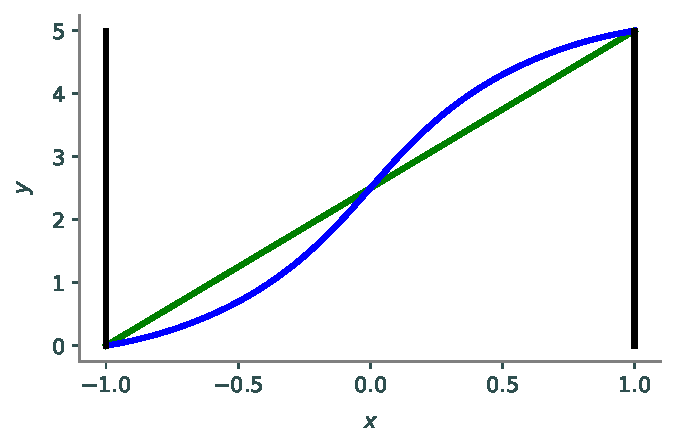
\includegraphics[width=\textwidth]{figures/minimum_time_rivercrossing.pdf}
\caption{Numerical computation of the trajectory with the shortest transit time.}
\label{fig:rivercrossing_trajectory}
\end{figure}



\begin{figure}[H]
\centering
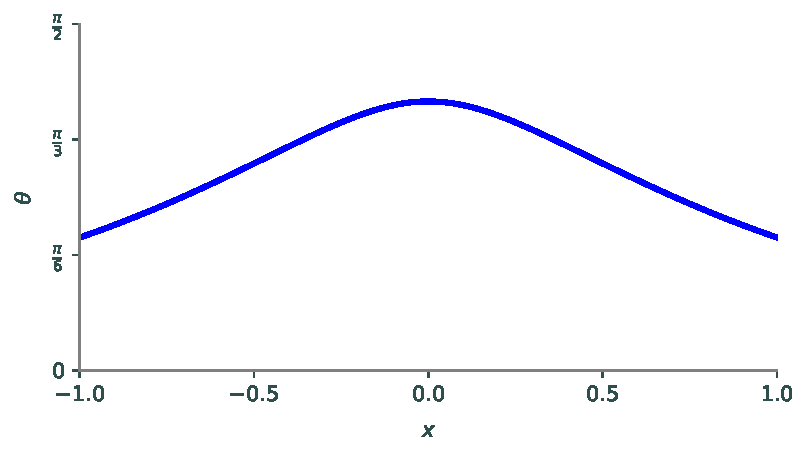
\includegraphics[width=\textwidth]{figures/trajectory_angle.pdf}
\caption{The optimal angle to steer the boat.}
\label{fig:rivercrossing_angle}
\end{figure}






